%You should title the file with a .tex extension (hw1.tex, for example)
\documentclass[12pt]{article}

\usepackage{fancyhdr, amsmath, enumerate, url, ulem, polynom, subfig,
  amssymb, amsthm, verbatim, graphicx,hyperref, booktabs, comment,
  listing}
\graphicspath{{/media/yujiex/work/computationGeometry/Computational-Geometry/tidyNotes/images/}}

\usepackage{proof}

\oddsidemargin0cm
\topmargin-2cm     %I recommend adding these three lines to increase the 
\textwidth16.5cm   %amount of usable space on the page (and save trees)
\textheight23.5cm  

\newcommand{\question}[2] {\vspace{.25in} \hrule\vspace{0.5em}
\noindent{\bf #1: #2} \vspace{0.5em}
\hrule \vspace{.10in}}
\renewcommand{\part}[1] {\vspace{.10in} {\bf (#1)}}

\newcommand{\myname}{Yujie Xu}
\newcommand{\myandrew}{yujiex@andrew.cmu.edu}
\newcommand{\myhwnum}{00}

\newcommand{\fref}[1]{Figure \ref{#1}}
\newcommand{\tref}[1]{Table \ref{#1}}
\newcommand{\eref}[1]{Equation \ref{#1}}

\setlength{\parindent}{0pt}
\setlength{\parskip}{5pt plus 1pt}

 
\pagestyle{fancyplain}
\lhead{\fancyplain{}{\textbf{Lecture Note}}}      % Note the different brackets!
\rhead{\fancyplain{}{\myname\\ \myandrew}}
\chead{\fancyplain{}{15-456}}

%
% The following macro is used to generate the header.
%
\newcommand{\lecture}[4]{
   \pagestyle{myheadings}
   \thispagestyle{plain}
   \newpage
   \stepcounter{#1}
   \setcounter{page}{1}
   \noindent
   \begin{center}
      \vbox{\vspace{2mm}
       \vspace{4mm}
       \hbox to 6.28in { {\Large \hfill Lecture \arabic{#1}: #2  \hfill} }
       \vspace{2mm}
       \hbox to 6.28in { {\it \hfill Instructor: #3 \quad Notes taken: Yujie Xu\hfill}}      
       \hbox to 6.28in { {\it  \hfill Date: #4 \hfill} }
      \vspace{2mm}}
   \end{center}
   \markboth{Lecture #1: #2}{Lecture \arabic{#1}: #2}
}

\newcommand{\hw}[4]{
   \pagestyle{myheadings}
   \thispagestyle{plain}
   \newpage
   \stepcounter{#1}
   \setcounter{page}{1}
   \noindent
   \begin{center}
      \vbox{\vspace{2mm}
       \vspace{4mm}
       \hbox to 6.28in { {\Large \hfill HW \arabic{#1}: #2  \hfill} }
       \vspace{2mm}
       \hbox to 6.28in { {\it \hfill Instructor: #3 \quad Notes taken: Yujie Xu\hfill}}      
       \hbox to 6.28in { {\it \hfill Date: #4} }
      \vspace{2mm}}
   \end{center}
   \markboth{Lecture #1: #2}{Lecture \arabic{#1}: #2}
}
%
% The following is my command for comments
%
\newcommand{\claim}[1]{\par {\bf Claim }{#1}}
\newcommand{\subclaim}[1]{\par {\bf Subclaim }{#1}}
\newcommand{\hp}[1]{\par {\bf HP: }{#1}}
\newcommand{\note}[1]{\par {\bf Note: }{#1}}
\newcommand{\rmk}[1]{\par {\bf Remark: }{#1}}
\newcommand{\que}[1]{\par {\bf Question: }{\it #1}}
\newcommand{\ans}[1]{\par {\bf Answer: }{\it #1}}
\newcommand{\eg}[1]{\par {\bf Examples: }{#1}}
\newcommand{\wn}[1]{\par {\bf Warning: }{#1}}

\begin{document}

\medskip                        % Skip a "medium" amount of space
                                % (latex determines what medium is)
                                % Also try: \bigskip, \littleskip

%
% The following commands set up the lecnum (lecture number)
% counter and make various numbering schemes work relative
% to the lecture number.
%
\newcounter{lec}
\renewcommand{\thepage}{\thelec-\arabic{page}}
\renewcommand{\thesection}{\thelec.\arabic{section}}
\renewcommand{\theequation}{\thelec.\arabic{equation}}
\renewcommand{\thefigure}{\thelec.\arabic{figure}}
\renewcommand{\thetable}{\thelec.\arabic{table}}

% Use these for theorems, lemmas, proofs, etc.
\newtheorem{theorem}{Theorem}[lec]
\newtheorem{lemma}[theorem]{Lemma}
\newtheorem{uf}[theorem]{Useful Fact}
\newtheorem{proposition}[theorem]{Proposition}
\newtheorem{corollary}[theorem]{Corollary}
\newtheorem{definition}[theorem]{Definition}
\newtheorem{remark}[theorem]{Remark}
\newtheorem{recall}[theorem]{Recall}
\newtheorem{fact}[theorem]{Fact}
%\newenvironment{proof}{{\bf Proof:}}{\hfill\rule{2mm}{2mm}}
%
% Convention for citations is authors' initials followed by the year.
% For example, to cite a paper by Leighton and Maggs you would type
% \cite{LM89}, and to cite a paper by Strassen you would type \cite{S69}.
% (To avoid bibliography problems, for now we redefine the \cite command.)
% Also commands that create a suitable format for the reference list.
\begin{comment}
\renewcommand{\cite}[1]{[#1]}
\def\beginrefs{\begin{list}%
        {[\arabic{equation}]}{\usecounter{equation}
         \setlength{\leftmargin}{2.0truecm}\setlength{\labelsep}{0.4truecm}%
         \setlength{\labelwidth}{1.6truecm}}}
\def\endrefs{\end{list}}
\def\bibentry#1{\item[\hbox{[#1]}]}
\end{comment}

%Use this command for a figure; it puts a figure in wherever you want it.
%usage: \fig{NUMBER}{SPACE-IN-INCHES}{CAPTION}
\newcommand{\fig}[3]{
			\vspace{#2}
			\begin{center}
			Figure \thelecnum.#1:~#3
			\end{center}
}

\par Template adapted from CMU's 10725 Fall 2012 Optimization course
taught by Geoff Gordon and Ryan Tibshirani.
%%

\pagebreak
\title{Note of Computer Graphics}
\maketitle

\lecture{lec}{Introduction, The Line Intersection Problem using
  Sweepline}{Gary Miller}{Monday, Aug 31, 2015}
\setcounter{section}{0}
\section{Intro}
\subsection{Course description from the syllabus}

``How do you sort points in space? What does it even mean? This course
takes the ideas of a traditional algorithms course, sorting,
searching, selecting, graphs, and optimization, and extends them to
problems on geometric inputs. We will cover many classical geometric
construc- tions and novel algorithmic methods. Some of the topics to
be covered are convex hulls, Delaunay triangulations, graph drawing,
point location, geometric medians, polytopes, configuration spaces,
computational topology, approximation algorithms, and others. This
course is a natural extension to 15-451, for those who want to learn
about algorithmic problems in higher dimensions.''

Textbook: Computational Geometry: Algorithms and
Applications~\cite{CG2008}.

Traditional algorithm courses mainly discuss 1D problems, such as
BST. The topics of this course contains the following main topics:
\begin{itemize}
\item Large dimensional problems
\item The change of the nature of simple geometry problems when
  dimension increases
\end{itemize}
The applications of computational geometry include:
\begin{itemize}
\item 2D: graphics
\item high dimension: machine learning
\item GIS
\item CAD, CAM
\item simulation
\end{itemize}
Algorithm design approaches:
\begin{itemize}
\item Divide and Conquer: ``Divide the problem on size n into k > 1
  independent subproblems on sizes $n_1 , n_2 , \dots n_k$ , solve the
  problem recursively on each, and combine the solutions to get the
  solution to the original problem.'' (15-210 lecture note)
\item 2D sweep-line
\item Random Incremental
\item 
\end{itemize}
The basic issues or standard computational problems that will be
discussed in recent lectures include:
\begin{itemize}
\item Line segment intersection (sweepline algorithm, random
  incremental algorithm)
\item Convex Hull: given a set of points, compute the convex hull of
  these points.
\item 2D-LP
\end{itemize}
The standard geometry problems that will be discussed recently
include:
\begin{itemize}
\item Line side test
\item In circle test
\end{itemize}
First the abstract objects and their representation that will be used
in this course are discussed and is listed in the \tref{tab:AO}
\begin{table}[h!]
\centering
\caption{Abstract Object and Their Representation}
\label{tab:AO}
\begin{tabular}{@{}l p{5cm}l@{}}
\toprule
Absract Object & Representation                                                                        & Issue          \\ \midrule
Real Number    & Float                                                                                 & Rounding Err   \\
               & Bignum (with arbitrary precision, normally they use arbitrary length array of digits) & Memory Intense \\
               & Computer Algebra (Symbolic Computation)                                               &                \\
Point          & Pair of Real                                                                          &                \\
Line           & Pair of Points                                                                        &                \\
Line Segment   & Pair of Points                                                                        &                \\
Triangle       & Tripple of Points                                                                     &                \\ \bottomrule
\end{tabular}
\end{table}
\section{How to use points to generate object}
Suppose $P_1, P_2, \dots P_k \in \omega^d$ where $P_k \in M$ is a
d-dimensional vector space with each point being a $M$-dimensional
point, the following combinations of points creates the linear
subspace of the vector space and generates geometric objects:
\begin{itemize}
\item \emph{Linear Combination}: 
$$Subspace = \sum_{i} \alpha_i \cdot P_i, \alpha_i \in \mathbb{R}$$ 

For the $d = 2$ and $P_i \in \mathbb{R}^3$ case, the linear
combination of $P_1$ and $P_2$ forms a plane with
$\vec{OP_1}, \vec{OP_2}$ being the basis.

\item \emph{Affine Combination}: 
$$Plane = \sum_{i} \alpha_i \cdot P_i, s.t. \; \alpha_i \in \mathbb{R} \land
\sum_{i} \alpha_i = 1$$ 

For the $d = 2$ and $P_i \in \mathbb{R}^3$ case, the affine
combination of $P_1$ and $P_2$ forms a line that passes $P_1, P_2$.

\item \emph{Convex Combination}: 
$$Body = \sum_{i} \alpha_i \cdot P_i, s.t. \; \alpha_i \in \mathbb{R} \land
\sum_{i} \alpha_i = 1 \land \alpha_i \geq 0$$

$S \subseteq \mathbb{R}^d$ is a convex set iff
$\forall p, q \in S \;\ldotp, [p, q] \subseteq S$ (A set S in a vector
space over R is called a convex set if the line segment joining any
pair of points of S lies entirely in S~\cite{convexSetWA})

For the $d = 2$ and $P_i \in \mathbb{R}^3$ case, the convex
combination of $P_1$ and $P_2$ forms a line segment between
$P_1, P_2$.

\emph{Convex Closure/Hull: } The minimal convex set $S' \supseteq S$ 

A subset $S$ of the plane is called convex if and only if for any pair
of points $p, q \in S$ the line segment $\overline{pq}$ is completely
contained in $S$. The convex hull CH(S) of a set S is the smallest
convex set that contains S~\cite{CG2008}.

\begin{theorem}
  $CC(P_1 \dots P_k) = \{\alpha \in \mathbb{R} \mid \sum_{i} \alpha_i
  = 1 \land \alpha_i \geq 0\}$

  In convex geometry Carathéodory's theorem states that if a point x
  of $\mathbb{R}^d$ lies in the convex hull of a set $P$, there is a
  subset $P'$ of $P$ consisting of $d + 1$ or fewer points such that x
  lies in the convex hull of $P'$.

\end{theorem}
\end{itemize}
\section{Primitives}
Problems related to geometry primitives
\begin{enumerate}[1)]
\item Test equality $p = q?$
\item Line segment intersection in 2D

  Let $L_1 = [P_1, P_2]$, $L_2 = [P_3, P_4]$, let
  $P_i = \begin{pmatrix}x_i \\ y_i\end{pmatrix}$.

  \begin{equation}\label{eq:lineSeg1}
    L_1 \cap L_2 \neq 0 \iff (P_1 P_2)\begin{pmatrix}\alpha_1 \\
      \alpha_2\end{pmatrix} = (P_3 P_4)\begin{pmatrix}\alpha_3 \\
      \alpha_4\end{pmatrix}
    \\\text{ and } \alpha_1 + \alpha_2 = \alpha_3 + \alpha_4 = 1 \text{ and }
    \alpha_i \geq 0.
  \end{equation}
  If written in matrix form, \eref{eq:lineSeg1} becomes:
  \begin{equation}\label{eq:lineSeg2}
    \begin{pmatrix}
      x_1 & x_2 & -x_3 & -x_4 \\
      y_1 & y_2 & -y_3 & -y_4 \\
      1 & 1 & 0 & 0 \\
      0 & 0 & 1 & 1 
    \end{pmatrix}
    \cdot
    \begin{pmatrix}
      \alpha_1\\
      \alpha_2\\
      \alpha_3\\
      \alpha_4\\
    \end{pmatrix}
    = 
    \begin{pmatrix}
      0\\
      0\\
      1\\
      1\\
    \end{pmatrix}
    \end{equation}
    So the general process of solving the line segment intersection
    problem is
    \begin{enumerate}[{Step }I.]
    \item Solve{eq:lineSeg2} with some solver
    \item Check if $\forall i, \alpha_i \geq 0$
    \end{enumerate}
    There could be more than one solutions when $L_1$ and $L_2$
    intersect in more than one point: the four point are collinear and
    there is an overlay. But in terms of the problem, the solution is
    still unique, since the solution is either True of False.
    
    \rmk{The good practice is make this line segment intersection test
      be a sum-routine and call an existing solver to solve the
      matrix. Don't try to inline the code}
    
    Some cases when the algorithm output False:
    \begin{itemize}
    \item $L_1$ and $L_2$ parallel but not collinear
    \item the intersection is on the extension of the two line segment
    \item the intersection is on one line segment and on the extension
      of the other.
    \end{itemize}

\item Line side test
  \begin{itemize}
  \item input: three points in 2D: $P_1, P_2, P_3$
  \item output: if $P_3$ is to the left of ray ${P_1P_2}$ 

    One process of solving the problem: Subtract $P_1$ from both of the
    other vectors.  Let $V_2 = P_2-P_1$ and $V_3 = P_3-P_1$.  Now the
    cross product $V_2 \times V_3$ is the signed area of the
    parallogram formed by $V_2$ and $V_3$.  This area is $>$ 0 if and
    only if $P_3$ is to the left of ray $P_1 \mapsto P_2$.
    
    Alternatively, suppose $P_1 = O$ (the origin), then the signed
    area of the parallogram formed by $\vec{P_1 P_2}, \vec{P_1, P_3}$
    is 
    \begin{equation}\label{eq:signArea}
      \det\begin{pmatrix}
        x_2 & x_3 \\
        y_2 & y_3 \\
      \end{pmatrix}
    \end{equation}

    \begin{equation}\label{eq:lineSideDet}
      LHS = \det\begin{bmatrix}
        x_1 & x_2 & x_2\\
        y_1 & y_2 & y_2\\
        1 & 1 & 1\\
      \end{bmatrix}
      =
      det\begin{bmatrix}
        x_1 & x_2 - x_1 & x_3 - x_1\\
        y_1 & y_2 - y_1 & y_3 - y_1\\
        1 & 0 & 0\\
        \end{bmatrix}
    \end{equation}
    Just report the sign of determinant of LHS of
    \eref{eq:lineSideDet}
  \end{itemize}
  \rmk{The good property of method 2 is that it can be generalized to
    higher dimension easily: for a 4D space, the test checks the
    determinant of a 4 by 4 matrix.}

\item In circle test
  \begin{itemize}
  \item input: four points in 2D: $P_1, P_2, P_3, P_4$
  \item output: if $P_4$ is in the circle of $(P_1, P_2, P_3)$
  \end{itemize}
\end{enumerate}

\section{Problems}
\subsection{Line Segment Intersection Problem}
\begin{itemize}
\item Input: n line segments
\item Output: All I intersections
\item Naive Approach: ${n \choose 2}$ line segment intersection
  tests. $O(n^2)$
\item There is $O(n\log n + |I|)$ today
\end{itemize}
\subsubsection{Sweep Line Algorithm}
Define the following:\
\begin{itemize}
\item Input: $S = \{S_1, \dots S_n\}$ line segments.
\item $P \equiv$ Line segment end points
\item $I \equiv$ Line segment intersections
\item $Event \equiv P \cup I$
\end{itemize}

Assumptions: 
\begin{itemize}
\item Horizontal line segments are not considered
\item The case where three lines intersect at the same point is not
  handled
\end{itemize}
$L$ is a horizontal line disjoint from $P \cup I$ that sweeps from top
to bottom\\

Linear ordering (transitive, irreflexive and total) $(A, \prec)$: 
\begin{itemize}
\item set $A = \{s \in S \mid s \cap l \neq \emptyset\}$
\item relation: the position of the intersection from left to right
  between line $L$ and the line segments:
  $p \prec q p_y > q_y \lor (p_y = q_y \land p_x < q_x)$
\end{itemize}
\rmk{Order of set A changes at events}

The order is stored in a Balanced BST B. The basic idea is to sweep the
line $L$ from top to bottom and stop at events.

\claim {if the next event is $S \cap S'$ then $S, S'$ are
neighbors}.

Priority queue $Q_L$ is kept to hold events. By induction, it contains:
\begin{itemize}
\item P below L
\item Neighboring line segments that intersect below $L$
\end{itemize}

Algorithm:
\begin{verbatim}
Insert P into Q
While Q not empty
P = ExtractMax(Q)
HandleEvent(P)

Handle Event(P):
    if P is upper end of S 
        insert (S, B)
        add-intersection(left(S), S, Q)
        add-intersection(S, right(S), Q)
    if P is lower end of S then
        add-intersection(left(S), right(S), Q)
        delete(S, B)
    if P is an intersection of S' and S
        swap (S, S', B)
        add-intersection(left(S'), S', Q)
        add-intersection(S, right(S), Q)
        report P
\end{verbatim}

Each step of the alg is $\log(n)$, there are n of upper end and lower
end. There are I of ``P is an intersection''. The total cost is $O(n +
|I|)\log n$

\subsubsection{Map Overlay Problem}
``given a set S of n closed segments in the plane, report all
intersection points among the segments in S''
\begin{itemize}
\item Input: segments $S = \{S_1, \dots, S_n\}$
\item Output: Break all segments into sub segments such that two sub
  segments intersect only at endpoints
\item Algorithm: SweepLine
\item Events: All segment intersections ($I$), and All end points ($P$)
\end{itemize}
Use link lists to store the following
\begin{itemize}
\item  $U(P) = $ Subsegments with the upper end point P
\item  $L(P) = $ Subsegments with the lower end point P
\item  $C(P) = $ intersection in P
\end{itemize}
First initialize U and L with S, initialize $C(P) = \emptyset$
The procedure goes as:\\
\texttt{HandleEvent(P point, T tree, Q queue)}
\begin{enumerate}[1)]
\item $\forall x \in C(P)$, form new sub segments, break S into $S_1,
  S_2$, add $S_1, S_2$ to $U(P)$ and $L(P)$
\item $\forall s \in L(P)$, delete (S, T)
\item $\forall s \in U(P)$, insert (S, T)
\item for all new neighbor pairs, add intersection to Q
\end{enumerate}
The run time of this algorithm is $O(m \log n)$ with
$m = \#subsegments$, because there's at most m inserts and deletes
into T and Q.

\lecture{lec}{Convex Hull-1}{Gary Miller}{Wed, Aug 31, 2015}
\setcounter{section}{0} 

Missed the lecture as a result of going to another lecture. The
following notes are tidied from the online lecture notes.
\section{Definitions}
\begin{definition}
  $A \subseteq \mathbb{R}^d$ is \emph{convex}, if it is closed under
  convex combination.
\end{definition}
\begin{definition}
  Convex Closure(A) $\equiv$ smallest convex set $\supseteq A$
\end{definition}
\begin{definition}
  \emph{Convex Hull}: 
  \begin{itemize}
  \item $CH(A) = JCC(A)$ (Boundary), we'll use this definition 
  \item $CH(A) = CC(A)$
  \end{itemize}
\end{definition}
$A$ is a finite set, thus in 2D, CH(A) is just a closed polygon with
vertices in counter-clockwise order.
\section{Lower Bound}
$Sorting \leq_M CH$: sorting problem reduces to convex hull problem,
meaning CH is at least as hard as sorting problem.
\begin{itemize}
\item Input: $(x_1, x_1^2), (x_2, x_2^2), \dots, (x_1, x_1^2)$
\item $CH(x_1, x_1^2), (x_2, x_2^2), \dots, (x_1, x_1^2)$ output a
  sequence of points with $x_i$ in sorted order.
\end{itemize}
\section{An important use of CH in triangulation}
Let $P_1, P_2, \dots P_n \in \mathbb{R}^2$,
$\bar{P_i} = (P_x, P_y, P_x^2 + P_y^2)$, then
$CH(\bar{P_1}, \bar{P_2}, \dots, \bar{P_n}) \equiv $ Triangulated
  surface, the \emph{Delaunay Triangulation}
 
  ``Triangulation is the division of a surface or plane polygon into a
  set of triangles, usually with the restriction that each triangle
  side is entirely shared by two adjacent
  triangles.''\url{http://mathworld.wolfram.com/Triangulation.html}

  To test whether a line segment is on convex hull or not, we'll use
  the following characterization:
  
\claim{[a, b] is on CH(A) iff $a \neq b$, and
  \begin{itemize}
  \item $a, b \in A$
  \item $\forall a' \in A$, either $a'$ left of [a, b] or $a' \in$ [a,
    b]
  \end{itemize}
}

\section{Quick Sort and Backward Analysis}
The process of quick sort is as follows:
\begin{verbatim}
QS(M):
    pick random a \in M
    split M with L < a < R
    return QS(L) * a * QS(R)
\end{verbatim}
Dart Game:
\begin{verbatim}
Initial state: an empty array of squares
while there exists an non-empty square
    pick a random non-occupied square to throw a dart on
\end{verbatim}
The cost of each dart throw is \# empty squares to the left of the
dart and the \# of empty squares to the right of the dart
\begin{claim}
  The expected cost of the dart game $=$
  the expected cost of quick sort
\end{claim}

Backward Dart Game:

\begin{verbatim}
Initial state: an array of squares each with a dart in it
while there exists a dart
    pick a random dart and remove it
\end{verbatim}

\begin{claim}
  The expected cost of the dart game $=$
  the expected cost of the backward dart game
\end{claim}

Analyzing the backward game:

Let $T_i$ be the expected cost of removing a random dart
\begin{figure}[h!]
  \centering
  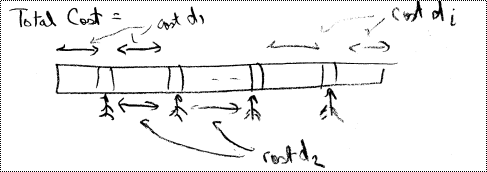
\includegraphics[width=0.4\linewidth]{dart.png}
  \caption{Backward Dart Game}
  \label{fig:dart}
\end{figure}
Each chunk of empty squares can be consumed by the dart on its left or
right, except for the left most and the right most chunk, so the total
cost of removing each of the $i$ dart is 
$$ \leq 2(n - i)$$
Averaging the total cost of the total $i$ possible event yields the
expected cost for removing a random dart when there are $i$ dart in
the board is:
$$T_i = {2(n - i) \over i}$$

The total expected cost of $i \in [1, n]$ is 
$$\sum_{i = 1}^n{2(n - i) \over i}$$
\section{Algorithms for CH}
\subsection{2D CH with Divide and Conquer}
\subsubsection{Procedure}
Let $A = \{P_1, P_2, \dots, P_n\}$, with $P_i = (x_i, y_i)$
Preprocess: sort points in A with x-coordinate.
\begin{listing}
2D-CH(A) = \\
\emph{if} $|A|$ = 1, return $P_1$ \\
\emph{else} $CH_L = 2D-CH(P_1, P_2, \dots, P_{n/2})$\\
            $CH_R = 2D-CH(P_{n/2 + 1}, \dots, P_{n})$\\
Stitch$(CH_L, CH_R)$
\end{listing}

\begin{verbatim}
a = rightmost(L)
b = leftmost(R)
LowerBridge(L, R)
    repeat the following:
    *) if lower_a is not left of (a, b) vector, set a <- lower_a
    **) if lower_b is not left of (a, b) vector, set b <- lower_b
UpperBridge(L, R)
    repeat the following:
    *) if upper_a is not right of (a, b) vector, set a <- upper_a
    **) if upper_b is not right of (a, b) vector, set b <- upper_b
\end{verbatim}
\begin{figure}[h!]
  \centering
  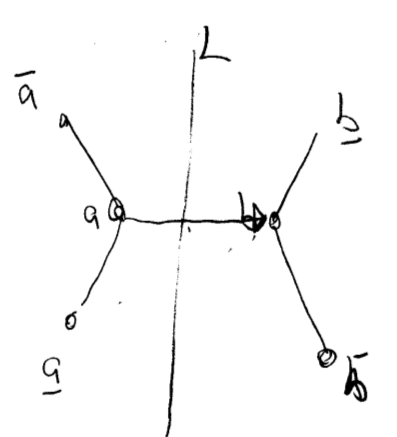
\includegraphics[width=0.4\linewidth]{stitch.png}
  \caption{stitch graph}
  \label{fig:stitch}
\end{figure}
\subsubsection{Correctness (Termination)}

Take \texttt{Lowerbridge} for example. Each step of *) or **) creates
a triangle, the triangles are ordered with the intersection of their
lowest point of intersection with the line L.

Each round of *) or **) moves one of a or b downwards and leaving the
intersection of the new edge, \texttt{lower\_a, b} or \texttt{a, lower\_b} with L strictly decreasing. There is a lower bound for the
edges $\{(x, y) \mid x \in L \land y \in R\}$.

Lower bridge is in $CC(A)$ by definition.

The proof for the upper bridge is symmetric to that of the LowerBridge.
\subsubsection{Cost}
Preprocess by sorting the point: $O(n \log n)$
\\Stitch is $O(n)$
\\$T(n) = 2T(n/2) + c \cdot n$, so the total cost is $O(n \log n)$

\subsubsection{Random Incremental CH}
The procedure of the Random Incremental goes as follows:
%Book Mark
\begin{verbatim}
Make a triangle T = (P1, P2, P3) from the set of points, 
pick a point C in the interior of T
Construct a ray from C to each of the Pi
Partition Pi by the edge of T they cross
Randomly permute P4 to Pn
    For i = 4 to n
    let e be edge crossed by ray c -> Pi
    BuildTent(P, e)

BuildTent(P, e):
    Find edges "visible" to P by searching out from e
    Replace visible edges with 2 new edges that are "just visible", i.e. one of their neighboring edges is not visible
    Assign rays to the new edges
\end{verbatim}

Runtime:\\
\begin{itemize}
\item Worst case: quadratic
\item Best Case: linear
\end{itemize}

Imaging all points are in counterclockwize order.

The worst case of this setting is the first triangle is
$(P_1, P_2, P_3)$ and new points come in sub-script increasing order,
for round 1, all the remaining $n - 3)$ points are partitioned to edge
$P_1, P_3$, then $BuildTent(P4, [P_1, P_3]$, nothing is visible
besides, $P_1, P_3$, do not add new edge, then go on, all edges are
partitioned to belong to $[P_1, P_4]$. For a stage with $i$ points in
the existing convex hull, $(n - i)$ partitioning operations are
needed, hence the total cost is $\sum_{i = 3} ^ n (n - i)$, which is
$O(n^2)$

\begin{figure}[h!]
  \centering
  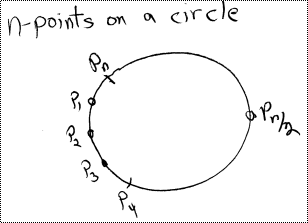
\includegraphics[width=0.4\linewidth]{randIncrWorst.png}
  \caption{Worst Case}
  \label{fig:randIncrWorst}
\end{figure}

The best case is, the first triangle is $(P_1, P_{n/2}, P_n)$. Half of
the points are assigned to $[P_3, P_{n/2}]$, the other half is
assigned to $[P_1, P_{n/2}]$. The work at the first stage is $n -
3$. Then BuildTent happens on the $P_{n/2}, P_{n/4}, P_{3n/4}, \dots$

Timing

\claim{Work other than BuildTent} cost $O(n)$

For BuildTent:
\begin{enumerate}[1)]
\item For each new point in $\{P_4, P_n\}$, there will be at most 2
  edges added, thus adding visible edges takes time at most 2n
\item For searching for ``visible'' edges: use amortized analysis with
  the following ``charging rule'':
  \begin{enumerate}
  \item If an edge $e$ is not visible, charge $P_i$, there are 2 for
    each $i$
  \item If an edge $e$ is visible, charge the edge. There are $4n$ of
    them, because the number of new edges added is $2n$, the number of
    removal of edges is also $2n$ (because an edge should be first
    added in order to be removed)
  \end{enumerate}
\item For step 3) of assigning rays to the two new edges in each stage.
  
Here we use the backward analysis. Consider on stage $i$ when there
are $i$ points ``processed'', we randomly pick one ``peg'' (point) and
remove it, if the peg is inside the rubber band boundary of the CH on
stage i, we cost nothing, if the rubber band changes, we spend the
number of rays crossing the left and right edge incident to the peg
that is just removed. i.e.

The cost of removing a random peg when there are $i$ pegs processed is 
$$P_i = 
\begin{cases}
  0 & P_i \text{ in interior}\\
  \# \text{rays crossing left or right} & \text{otherwise}\\
\end{cases}$$

The expected cost of removing a random peg on stage when there are
$i$ pegs not removed is: 
$$E_i \leq {2(n - i) \over i - 3}$$
The total cost is:
$$T = \sum_{i = 4}^n E_i \leq \sum_{i = 4}^n {2(n - i) \over i - 3}
\leq 2n \sum_{i = 1}^{n-3} {1 \over i} \leq 2n \sum_{i = 1}^n {1 \over
  i} = 2n H_n \in O(n \log n)$$
  
\end{enumerate}
\lecture{lec}{2D LP}{Gary Miller}{2015} 

\section{Introduction}
The problem that given Half space (Hspace) $H_1, H_2, \dots, H_n$, to
compute the intersection is equivalent to sorting and it takes $O(n
\log n)$: 
$$\bigcap{H_i} \equiv Sorting$$
Although sorting takes $O(n \log n)$, the ``selection'' problem takes
only $O(n)$. The same goes with the ``selection'' version of the Half
space intersection problem, which is to find the farthest point in
some direction.

\begin{definition}
  LP: maximize $C^T x$ subject to $Ax \leq d$ where $A$ is a
  $n \times m$ matrix in $\mathbb{R}^{n \times m}$,
  $x, C \in \mathbb{R}^ {m \times 1}$, $d \in {n \times 1}$. Define
  $x < y$ if $\forall i \;\ldotp x_i < y_i$
\end{definition}

\begin{definition}
  The LP is \emph{feasible} if $\exists x \;\ldotp Ax \leq d$ \note
  {the region $\{x \mid Ax \leq d\}$ is convex.}
\end{definition}
For the 2D case, 
$$\begin{pmatrix} a_1 & b_1 \\ \vdots \\ a_n & b_n \end{pmatrix}
  \begin{pmatrix} x \\ y \end{pmatrix} = 
  \begin{pmatrix} d_1 \\ \vdots \\ d_n \end{pmatrix}
$$
\emph{Geometric View of half plane}\\
$a_i x + b_i y \leq d$ with $d \geq 0$ is a half plane normal to the
vector $(a_i, b_i)$
\begin{figure}[h!]
  \centering
  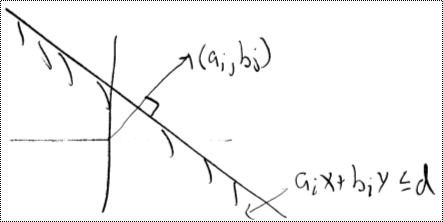
\includegraphics[width=0.5\linewidth]{hplane.png}
  \caption{The half plane geometric view}
  \label{fig:hplane}
\end{figure}

\emph{Input}: Half Space, $\{H_1, \dots, H_n\}$ and a vector $C \in \mathbb{R}^2$.
\pagebreak

\emph{Goal}: to find the $x \in \bigcap_{i = 1}^n H_i$ farthest in C
direction.

\emph{Simplifications}:
\begin{enumerate}[1)]
\item No $H_i$ normal to C, (unique OPT solution)/
\item Bounded feasible solutions (not saying the $\bigcap_{i = 1}^n
  H_i$ is bounded, but it is bounded in the C direction).
\item Given a ``Bounding Box'': $m_1, m_2$.
  \begin{figure}[h!]
    \centering
    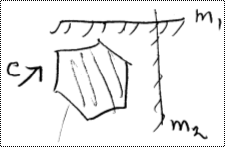
\includegraphics[width=0.5\linewidth]{bbox.png}
    \caption{Bounding Box}
    \label{fig:bbox}
  \end{figure}
\end{enumerate}
\section{1D LP}
\begin{itemize}
\item Input: Constraints in the form $a_ix \leq b_i, a_i \neq 0$
\item WLOG $a_i = 1$
\item Constraints can be classified into two categories:
  \begin{itemize}
  \item $C^+ = \{i \mid x \leq b_i\}$ (UB)
  \item $C^- = \{i \mid -x \leq b_i\}$ so $x \geq -b_i$ (LB)
  \end{itemize}
  Define $\alpha = \max \{-b_i \mid i \in C^-\}$ and $\beta = \{b_i
  \mid i \in C^+\}$
  \note{Feasible if $\alpha \leq \beta$}
    
  \item If feasible, return $\beta$ if $sign(C) = 1$, return $\alpha$
    otherwise.
\end{itemize}
\begin{theorem}{1D-LP is $O(n)$}
\end{theorem}
Because find max or min is $O(n)$
\section{2D LP}
The idea is to bring in\emph{random} constraint one at a time and
update the solution.
\subsection{Procedure}
\begin{verbatim}
v0 <- 2D-LP(m1, m2, c) = \partial(m1) \land \partial(m2) --- (*)
randomly order h1, ... , hn
for i = 1 to n do
    if v(i-1) \in hi then vi <- v(i - 1)                 --- (*)
    else (make and solve 1D-LP)
        L = \partial(hi)
        L1' = L \cap h1, ..., L_{i - 1}' = L \cap h_{i - 1}
        C' = proj(C, L) , note C' \neq 0
        vi = 1D-LP(h1', ..., h{i - 1}', C')              --- (*)
    if vi is undefined, report "no-solution" and halt.
\end{verbatim}
\subsection{Correctness}
\begin{claim}
  At the time marked with (*), $v_i = LP(m_1, m_2, h_1, \dots, h_i, C)$
\end{claim}
\begin{proof} by induction
  \begin{itemize}
  \item Base Case: OK by definition of bounding box.
  \item Inductive Case: assume $v_{i - 1}$ is correct.
    \begin{enumerate}[{Case }i]
    \item $v_{i - 1} \in h_i$, then $v_{i - 1} \in $ feasible region,
      so $v_{i - 1}$ is OPT for $h1, \dots, h_i$
    \item $v_i \notin h_i$
      \claim{$v_i \in \partial{h_i} = L$}
      \begin{proof}
        Assume for the sake of contradiction, $v_{i}$ is inside $L$,
    say the line segment $[v_i, v_{i - 1}$ intersect $L$ at A, then
    according to the previous assumption, there is always unique
    solutions to the LP, so from $v_{i - 1}$ to A to $v_i$, the
    objective value strictly decreases. thus the objective value at A
    is greater than that at $v_i$ and A is feasible. Hence the
    assumption that $v_i$ is inside $L$ is false.
      \end{proof}
      Still need to show why solving 1D LP will give the right
      solution.
    \end{enumerate}
  \end{itemize}
\end{proof}
\subsection{Timing}
\claim{2D LP is $O(n)$ expected time}
We use backwards analysis by randomly throw away some constraints.

For a stage with i constraints: $h_1, \dots, h_i$, we remove some
random constraints $h_j$.
\begin{definition}
  $h_j$ is \emph{critical} if removing it changes the OPT
  solution. There are at most 2 critical constraints at each point
  $v_i$ (the OPT for the stage where there are $i$ constraints)
\end{definition}
Cost of removing $h_j = k$ if $h_j$ is not critical, $k \cdot i$
otherwise. $k$ is some constants. (why??)

The worst case is when there are exactly 2 critical constraints.
$$E_i = {2 \cdot ki + (i - 2)k \over i} \leq {3ki \over i} = 3k$$
The total expected cost is $\sum_{i = 1}^n 3k = O(n)$

\section{Finding the Bounding Box}
\subsection{Definitions and theorems}
\begin{theorem}
  The LP is unbounded or we can find the bounding box.
\end{theorem}

\begin{lemma}
  $Ax \leq b$ maximize $C^T x$ is unbounded iff
  \begin{enumerate}[1)]
  \item The LP is a feasible
  \item $\exists d \;\ldotp C^T d > 0 \land Ad \leq 0$ (this is to
    slide the lines to the origin)
  \end{enumerate}
\end{lemma}
\begin{proof} ($\impliedby$)\\
  By 1) we can pick $x \in \mathbb{R}^{m \times 1}$ s.t. $Ax \leq b$

  By 2) we can find $d \in \mathbb{R}^{m \times 1}$ s.t. $C^T d \geq
  0$ and $Ad \leq 0$.
  
  \claim{$\alpha d + x$ is feasible and can be arbitrarily large}

  \begin{proof}
  $A(\alpha d + x) = \alpha A d + A x \leq Ax + b \leq b$ for all
  $\alpha \geq 0$, so for all $\alpha \geq 0$, $\alpha d + x$ is
  feasible.
  
  $C^T(\alpha d + x) = \alpha C^T d + C^T x$ can be arbitrarily large.
  \end{proof}
\end{proof}
\begin{proof} ($\implies$) \\
  (Hint: using the compactness argument)

  First, since the LP is unbounded, by definition, it is feasible.
  
  There exists $x_1, x_2, \dots$ such that $A x_i \leq b$ and
  $\lim_{i \to \infty} C^T x_i = \infty$. Let
  $S = \{d \mid C^T d > 0\} \neq \emptyset$ (??)
\end{proof}

\subsection{Procedure to find d}
WLOG, $\exists d$ s.t. $C^T d = 1$ and $Ad \leq 0$ is projected rows
of A onto line $C^T x = 1$. (slide all constraints so that they pass
the origin) and solve the 1D LP.
\note{$\exists d \iff \beta \geq \alpha$}
\begin{enumerate}[{Case }i]
\item {$\beta < \alpha$ then $Ax \leq b$ is feasible, thus $C^T x$
  subject to $Ax \leq b$ is unbounded}
\item {$\beta = \alpha$ then either the LP is not feasible, or it is
  unbounded (because there are two parallel constraints}
\item $\alpha < \beta$, then $h_\alpha \equiv$ half Space giving
  $\alpha$, and $h_\beta \equiv$ half space giving $\beta$. $h_\alpha,
  h_\beta$ are the bounding box.
\end{enumerate}

\lecture{lec}{Geometric Transformation}{Gary Miller}{Monday, Sep 09,
  11, 2015}
\section{General Intro}
The geometric transformation is related to the following problems:
\begin{itemize}
\item Linear Programming
\item Convex Hull
\item Delaunay Triangulation
\item Voronoi Diagram
\item Stereographic Map
\end{itemize}

\section{Definitions}
\begin{definition}
$\mathbb{R}^d$ is a \emph{d-dimensional} real space. A point p in a
d-dimensional space is written as $p = \begin{bmatrix} P_1 \\ \vdots \\
  P_d \end{bmatrix}$\\
$||p||^2 = P_1^2 + \dots + P_d^2 = P^TP = \begin{bmatrix}P_1 & \dots &
  P_d\end{bmatrix} \begin{bmatrix} P_1 \\ \vdots \\ P_d \end{bmatrix}$
\end{definition}

\begin{definition}
\emph{Hyperplane}: $\{x \in \mathbb{R}^d \mid P^T X = \alpha\}$ \\
\emph{Halfplane}: $\{x \in \mathbb{R}^d \mid P^T X \leq \alpha\}$ \\
The P vector is the normal vector to the plane.
\end{definition}

\begin{definition} (Reflection about unit sphere)
$$Reflect(P) = {P \over P^T P} = {P \over |P|^2}$$
\end{definition}
\rmk{$P \in$ unit sphere (on the boundary) are fixed points, i.e. $P^T
P = 1$}
\rmk{points inside the unit sphere is sent to the outside}
\rmk{points outside the unit sphere is sent to the inside}

\lecture{lec}{Guarding a Polygon}{Gary Miller}{Friday, Sep 25, 2015}
\section{Guarding a Polygon}
\begin{itemize}
\item Input: Polygon P.
\item Output: k ``guards'' $p_1, \dots, p_k$ inside P so that for all
  points of P, there exist a guard that can see it. i.e. we want
  \begin{itemize}
  \item k guards that cover P
  \item k is small
  \end{itemize}
\end{itemize}
\begin{theorem}
  For a polygon P with n vertices, ${n \over 3}$ guards are necessary
  (\fref{fig:guard}) and sufficient to cover P.
\end{theorem}
\begin{figure}[h!]
  \centering
  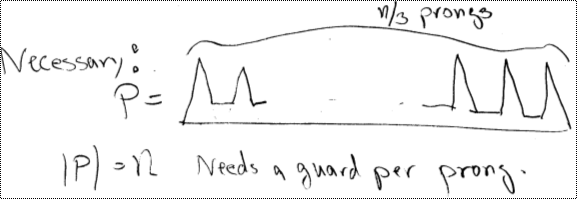
\includegraphics[width=0.5\linewidth]{guard.png}
  \caption{The case when $3/n$ guards are needed}
  \label{fig:guard}
\end{figure}
\bibliographystyle{plain} \pagebreak

\bibliography{Bibliography}
\end{document}